\documentclass[12pt,titlepage]{article}

% This first part of the file is called the PREAMBLE. It includes
% customizations and command definitions. The preamble is everything
% between \documentclass and \begin{document}.

\usepackage[margin=1in]{geometry}  	% set the margins to 1in on all sides
\usepackage{setspace} \doublespacing 	% double spaced
\usepackage{graphicx}              			% to include figures
\usepackage{epstopdf}
\usepackage{amsmath}               		% great math stuff
\usepackage{amsfonts}              		% for blackboard bold, etc
\usepackage{amsthm}                		% better theorem environments
\usepackage[numbers]{natbib}			% for bibiliography with numbers
\usepackage{hyperref}				% make link clickable


%%%%%%%%%%%%%%%%%%%%%%%%
% Document Begins Here %
%%%%%%%%%%%%%%%%%%%%%%%%

\begin{document}

\begin{titlepage}
    \begin{center}
        \vspace*{1cm}


        {\scshape\Large CMPUT681\par}
        {\scshape\LARGE Parallel and Distributed Systems\par}   
        \vspace{0.5cm}
        {\scshape\Large Project Report - Fall 2022\par}
        \vfill
        
        %%%% PROJECT TITLE
        \Huge
        \textbf{The eXpress Data Path\\}
        \LARGE
        Fast Programmable Packet Processing in the Operating System Kernel

        \vfill

        %%%% AUTHOR(S)
        {\Large Naveenraj Muthuraj\par}
        {\Large nmuthura@ualberta.ca \par}
        {\Large 1769237 \par}

    \end{center}
\end{titlepage}

\doublespacing
\tableofcontents
\singlespacing

\newpage

\doublespacing


\section{Introduction}

Network stacks in general purpose operating systems are typically optimised for flexibility. 
This means they perform too many operations per packet, this will eventually lead to bottleneck in network performance  since the network devices and interfaces nowadays come with high speed packets rates upto 100Gbps . This has led to the increasing popularity of software packet processing, such as Data Plane Development Kit (DPDK) \cite{dpdk}. These tools are implemented using kernel bypass techniques, where a userspace application takes complete control of the networking hardware to avoid expensive context switch between kernel and userspace. 

While the kernel bypass approach can significantly improve performance it has its own drawbacks. Firstly, It is difficult to integrate with existing system. Secondly the applications have to re-implement functionality otherwise provided by the operating system network stack, 
such as routing tables and higher level protocols. Lastly, userspace application implementing entire networking stack will increase complexity and blurs security boundaries otherwise enforced by the operating system kernel. 

To overcome these drawbacks of kernel bypass design. \citet{xdp} presented a system that adds programmability directly in the operating system networking stack in a cooperative way. This makes it possible to perform high-speed packet processing that integrates seamlessly with existing systems, while selectively leveraging functionality in the operating system. This framework, called the eXpress Data path (XDP). 

In this report we present a brief introduction to XDP and the results of reproducing the experiments originally conducted by \citet*{xdp}. 
This is structured as follows: Section 2 brief note on XDP, Section 3 experiment Setup and Section 4 presents performance evaluation in comparison to original study and Section 5 concludes with lessons learnt.

\section{The XDP}

eXpress Data Path (XDP) works by defining a limited execution environment in the form of a virtual machine running eBPF code, an extended version of original BSD Packet Filter(BPF) \cite{mccanne_bsd_1993} byte code format.  
It \textit{"BPF is eating the software"}\footnote{\href{https://blog.cloudflare.com/cloudflare-architecture-and-how-bpf-eats-the-world/}{Cloudflare - How eBPF eats the world}} 


\section{Experiment Setup}

Talk about  RFC 2544 \cite{rfc2544} for Network benchmarking .

Insert Experiment Setup Diagram 

\subsection{Considerations}


\begin{table}[]
\begin{tabular}{|l|r|r|r|r|l|}
\hline
\textbf{Instance Type} & \multicolumn{1}{l|}{\textbf{NIC}} & \multicolumn{1}{l|}{\textbf{NIC Queues}} & \multicolumn{1}{l|}{\textbf{CPU}} & \multicolumn{1}{l|}{\textbf{Memory}} & \textbf{Network Bandwidth} \\ \hline
\textit{c5n.large}     & 3                                 & 2                                        & 2                                 & 5.25                                 & Up to 25 Gigabit           \\ \hline
\textit{c5n.xlarge}    & 4                                 & 4                                        & 4                                 & 10.5                                 & Up to 25 Gigabit           \\ \hline
\textit{c5n.2xlarge}   & 4                                 & 8                                        & 8                                 & 21                                   & Up to 25 Gigabit           \\ \hline
\textit{c5n.4xlarge}   & 8                                 & 16                                       & 16                                & 42                                   & Up to 25 Gigabit           \\ \hline
\textit{c5n.9xlarge}   & 8                                 & 32                                       & 36                                & 96                                   & 50 Gigabit                 \\ \hline
\textit{c5n.18xlarge}  & 15                                & 32                                       & 72                                & 192                                  & 100 Gigabit                \\ \hline
\end{tabular}
\caption{AWS Network Optimised Instances and their Network Specifications}
\label{tab:aws-table}
\end{table}


Talk about all the environment that was considered and why you ended up choosing AWS . Use this Table~\ref{tab:aws-table} to explain the aws instances

\subsection{Limitations}

Talk about the limitation of Cloud based instances and restriction of network interface cards. All the pitfalls the was faced

\section{Performance Evaluation}


\begin{figure}
	\begin{center}
		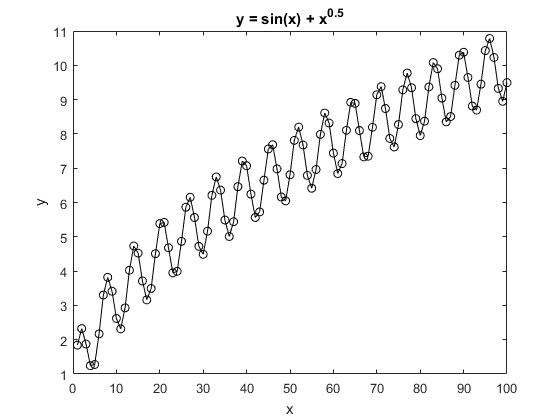
\includegraphics[scale=0.9]{img/plot.png}
	\end{center}
	\caption{Probability of including [k] faulty/malicious nodes in the service}
	\label{graph:sample-plot}
\end{figure}

For example, Figure~\ref{graph:sample-plot} compares the performance of XDP and Linux

\section{Conclusion}

XDP is faster


%%%%%%%%%%%%%%%%%%%%%%%%
% Bibliography Begins Here %
%%%%%%%%%%%%%%%%%%%%%%%%


\begin{spacing}{1}
\bibliographystyle{plainnat}
\bibliography{xdp_report}
\end{spacing}

\end{document}
